\section{Quantum Modular\\ Exponentiation}
\label{sec:modexp}

We now extend our arithmetic to modular exponentiation, which is repeated
modular multiplication controlled on qubits supplied by a phase estimation
procedure.
If we wish to multiply a $n$-qubit quantum input number $\ket{x}$ by
$t$ classical numbers $a^{(j)}$, we can multiply them in series.
% as shown in
%Figure \ref{fig:modexp-qc-series}.
This requires depth $O(t\log n)$ based on the modular multipliers in previous
sections.

%\begin{figure}[htp!]
%\begin{center}
%\includegraphics[width=5.5in]{figures/modexp-qc-series.pdf}
%\end{center}
%\caption{Multiplying a quantum number $\ket{x}$ by $t$ classical numbers
%$\{a^{0}, a^{1}, \ldots, a^{n-1}\}$ in series.}
%\label{fig:modexp-qc-series}
%\end{figure}

Now consider the same procedure, but this time each classical number $a^{(j)}$
is controlled on a quantum bit $p_j$. This is a special case of
multiplying by $t$ quantum numbers in series, since a classical number
entangled with a quantum number is also quantum.
%This is shown in
%Figure \ref{fig:modexp-qq-series}.
It takes the same depth $O(t\log n)$ as the previous case.
%
%\begin{figure}[htp!]
%\begin{center}
%\includegraphics[width=5.5in]{figures/modexp-qq-series.pdf}
%\end{center}
%\caption{Multiplying a quantum number $\ket{x}$ by $t$ quantum numbers
%$\{\ket{a^{0}p_0}, \ket{a^{1}p_1}, \ldots, \ket{a^{n-1}p_{n-1}}\}$ in series.}
%\label{fig:modexp-qq-series}
%\end{figure}

Finally, we consider multiplying $t$ quantum numbers
$\{x^{(0)}, x^{(1)}, \ldots, x^{(n-1)}\}$ in a parallel,
logarithmic depth, binary tree.
This is shown in Figure \ref{fig:modexp-qq-parallel}.
The tree has depth $\log_2(t)$ in modular multiplier operations. Furthermore,
each
modular multiplier operation has depth $O(\log(n))$ for $n$-qubit
numbers. Therefore, the overall depth of this parallel modular exponentiation
structure is $O(\log(t)\log(n))$. In phase estimation for QPF, it is
sufficient to take $t = O(n)$ \cite{Nielsen2000,Kitaev2002}. Therefore our total depth is
$O(\log^2(n))$ as desired. At this point, combined with the parallel phase
estimation procedure of \cite{Kitaev2002}, we have a complete factoring
implementation in our 2D nearest-neighbor architecture.
%
\begin{figure*}[tb!]
\centerline{
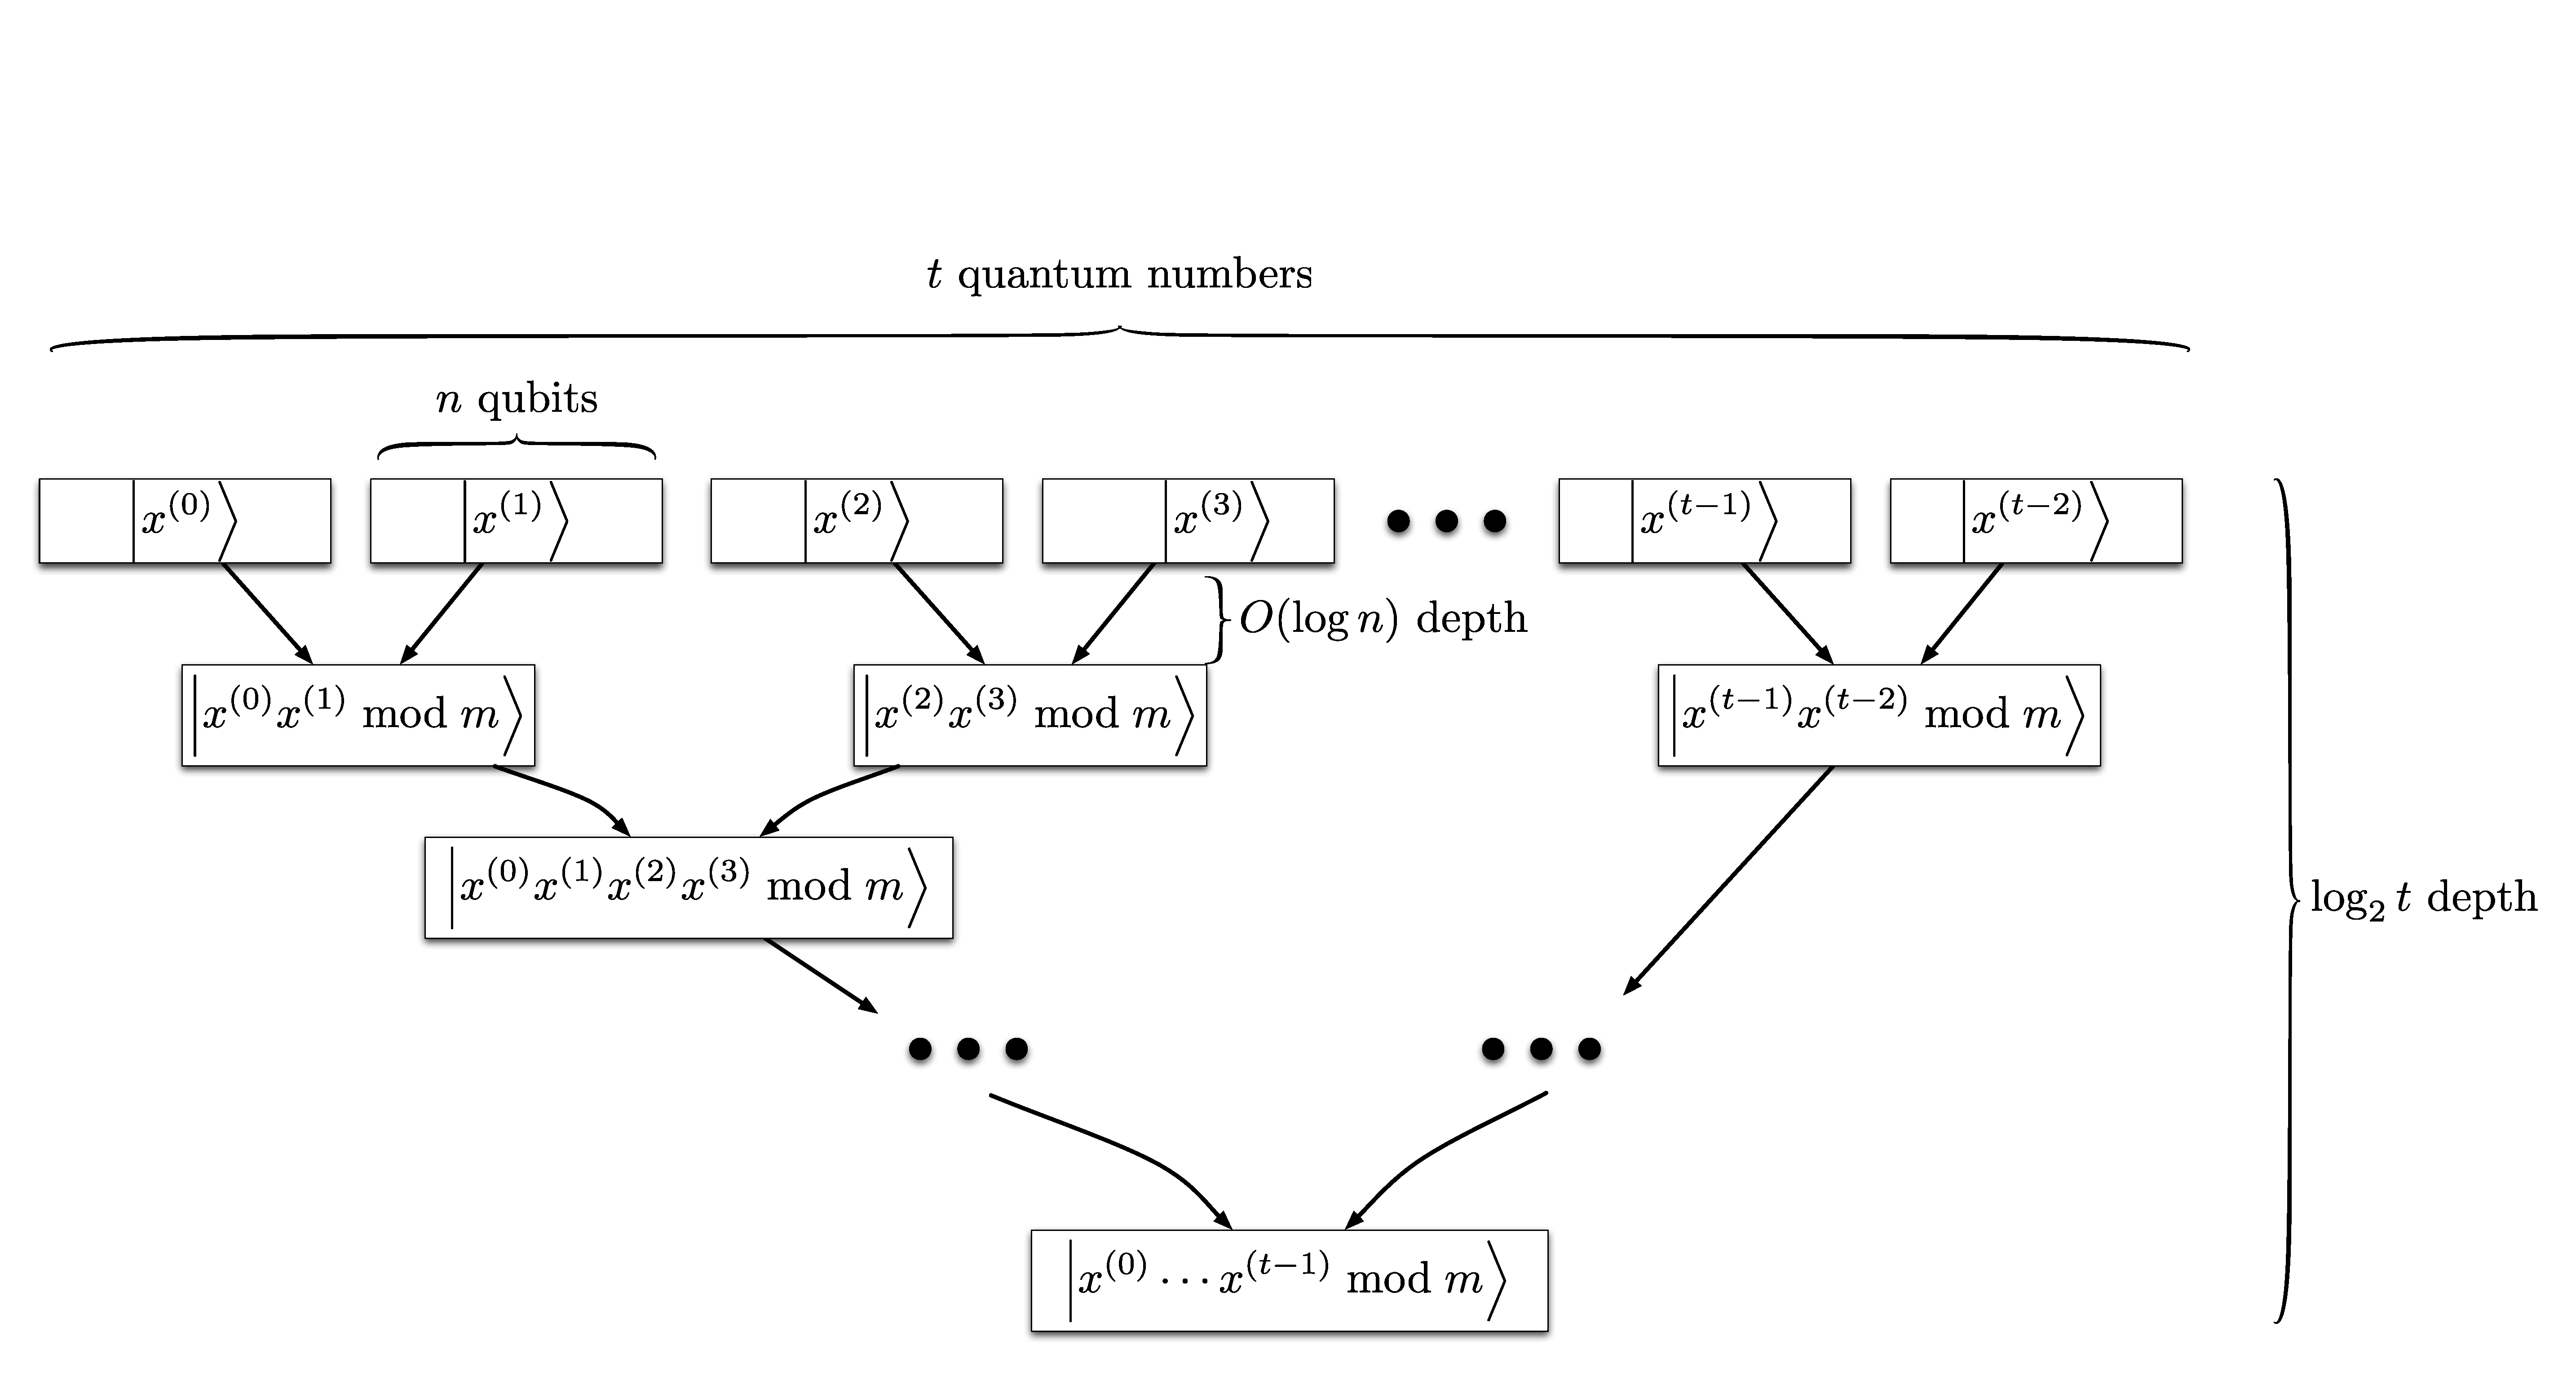
\includegraphics[width=5.5in]{figures/mod-exp-par.pdf}
}
\caption{Parallel modular exponentiation: multiplying $t$ quantum numbers
%$\{\ket{x^{(0)}}, \ket{x^{(1)}}, \ldots, \ket{x^{(t-1)}}\}$ in parallel,
in a $O(\log{(t)}\log{(n)})$-depth binary tree.}
\label{fig:modexp-qq-parallel}
\end{figure*} 

For all known QPF procedures, there are $t=O(n)$ control bits needed, and
also $O(n)$ modular multiplications in a tree of depth $O(\log n)$.
Each modular multiplication has
depth $O(\log n)$ and width $O(n^3)$.
Therefore, the depth of the parallel modular exponentiation circuit above
is $O(\log^2 n)$ and the width is $O(n^4)$.
